As for decentralized training, each agent is represented by its own network (and therefore optimizer, during training). This means that each agent's network is being fitted only to its own actions, rewards and observations, rather than their collective counterparts. This approach can benefit training because when using the collective reward and observation, centralized networks might not be able to capture small changes in actions for each agent. Furthermore, this in turn allows us to use Social Influence, a concept in which each agent's behavior is influenced by others, which we will further explain. 

The key concept is that we are using this neural network as a universal function approximator in order to approximate our theoretical $Q$ function, which we could use to pick the maximum value action for each state. We assume the fact that every $Q$ function obeys the \textit{Bellman Equation}:
\[
Q^\pi(s, a) = r + \gamma Q^\pi(s', \pi(s'))
\]
From this, we get the temporal difference error, $\delta$, which is what we attempt to minimize:
\[
\delta = Q(s, a) - \left(r + \gamma \max_{a'} Q(s', a')\right)
\]

The training pipeline for this approach follows closely \cite{pytorchrltutorial}. Each agent is represented by its own policy network and target network. We select actions according to an epsilon greedy policy, using Replay Memory to store transitions of the type \textit{(State, Action, Next State, Reward}. By obtaining a batch of these transitions for each autonomous agent, we optimize the network by minimizing the \textit{Huber Loss} calculated with respect to the previously mentioned $delta$:

\[
L = \frac{1}{|B|} \sum_{(s, a, s', r) \in B} L(\delta),
\]
where
\[
L(\delta) =
\begin{cases} 
\frac{1}{2}\delta^2 & \text{for } |\delta| \leq 1, \\
|\delta| - \frac{1}{2} & \text{otherwise}.
\end{cases}
\]

where $(s, a, s', r)$ is a single transition.

Having succesfully achieve decentralized training, the next step would be to implemented some kind of social mechanism, given that the agent's have to learn to respond to each other's behavior, in particular in an road intersection scenario. We chose to implement what is known as the \textit{Basic Social Influence} mechanism from \cite{jaques2019social}, that shifts agent's rewards using counterfactuals, so that it becomes $r^k_t = \alpha e^k_t + \beta c^k_t$ where $e^k_t$ is the extrinsic or environmental reward, and $c^k_t$ is the causal influence reward.  Essentially, agent \textit{k} asks the question: “How would \textit{j’s} action change if I had acted differently in this situation?”. This causal influence rewards is obtained by calculating the divergence between the marginal policy of j (if \textit{j} did not consider \textit{k}) and the conditional policy of \textit{j} (when \textit{j} does consider \textit{k}).

\begin{figure}[h]
    \centering
    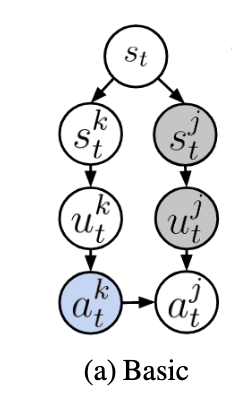
\includegraphics[scale=0.5]{images/social_influence.png}
    \caption{Chain of social influence}
    \label{fig:social influence}
\end{figure}